\documentclass[11pt]{article} 
\usepackage{setspace} 
\usepackage{amsmath}
\usepackage{booktabs}
\usepackage{graphicx}
\usepackage[colorlinks=true, linkcolor=black]{hyperref}
\usepackage[backend=biber,style=apa]{biblatex} % Use APA style, adjust as needed
\addbibresource{references.bib}




\setstretch{1.5} 

\title{Estimating House Prices in India}
\author{Ori Lipper \and Yonatan Lahat}
\date{06.12.2024}


\begin{document}
\maketitle




\begin{abstract}
Predicting house prices is a complex challenge with significant implications for real estate markets and stakeholders. This study employs data-driven methodologies to analyze key determinants of house prices and develop predictive models. Exploratory Data Analysis (EDA) revealed that structural features such as \texttt{Total\_Area}, \texttt{living area}, and \texttt{grade of the house} are the strongest positive contributors, while factors like \texttt{House\_Age} and \texttt{Time\_Since\_Renovation} negatively impact prices. Using an Ordinary Least Squares (OLS) regression model, we explained 64.2\% of the variance in house prices, achieving a Mean Absolute Error (MAE) of \$130,064 and a Root Mean Squared Error (RMSE) of \$234,642 on test data. 

Despite reasonable performance, the model faced challenges with multicollinearity, heteroscedasticity, and residual non-normality, particularly for higher-priced properties. Influential observations further underscored the need for robust outlier handling. The study discusses the limitations and proposes future improvements, including advanced modeling techniques, feature engineering, and integration of neighborhood-level and market data. These findings highlight the potential of data-driven approaches for more accurate and interpretable real estate price prediction.
\end{abstract}


\section{Introduction}

Understanding the factors that influence house prices is a critical challenge in real estate analytics. Accurate prediction models not only assist in market evaluation but also empower stakeholders to make informed decisions. This paper explores the application of data-driven methodologies to analyze and model housing prices, leveraging statistical and machine learning techniques.

We begin with Exploratory Data Analysis (EDA) to uncover patterns, relationships, and anomalies in the dataset. This stage lays the groundwork for data cleaning, feature engineering, and hypothesis generation. Key features such as \texttt{Living Area}, \texttt{Number of Bedrooms}, and \texttt{Bathrooms} are examined for their impact on property value. Statistical testing and correlation analysis further refine our understanding of feature importance.

The core of this study is the construction of regression models to predict house prices. Using Ordinary Least Squares (OLS) regression as a baseline, we quantify the contributions of significant predictors and assess the model's performance through metrics such as \(R^2\), Mean Absolute Error (MAE), and Root Mean Squared Error (RMSE). Model diagnostics, including residual analysis and multicollinearity evaluation, are employed to ensure robustness and reliability.

This paper aims to provide a comprehensive framework for analyzing housing data, balancing interpretability with predictive accuracy. By addressing common challenges such as data skewness, outliers, and feature redundancy, we demonstrate the potential of data-driven approaches in solving real-world problems in the housing market.




\section{Results}

\subsection{Exploratory Data Analysis (EDA)}

EDA explores dataset characteristics to uncover patterns, anomalies, and relationships. Key steps include analyzing the target variable (\texttt{Price}) distribution, feature relationships, and data preparation.

\subsubsection{Target Variable Distribution}
The \texttt{Price} distribution is right-skewed, with most values in the lower range. A logarithmic transformation may address skewness for better model fit.

\begin{figure}[htbp]
    \centering
    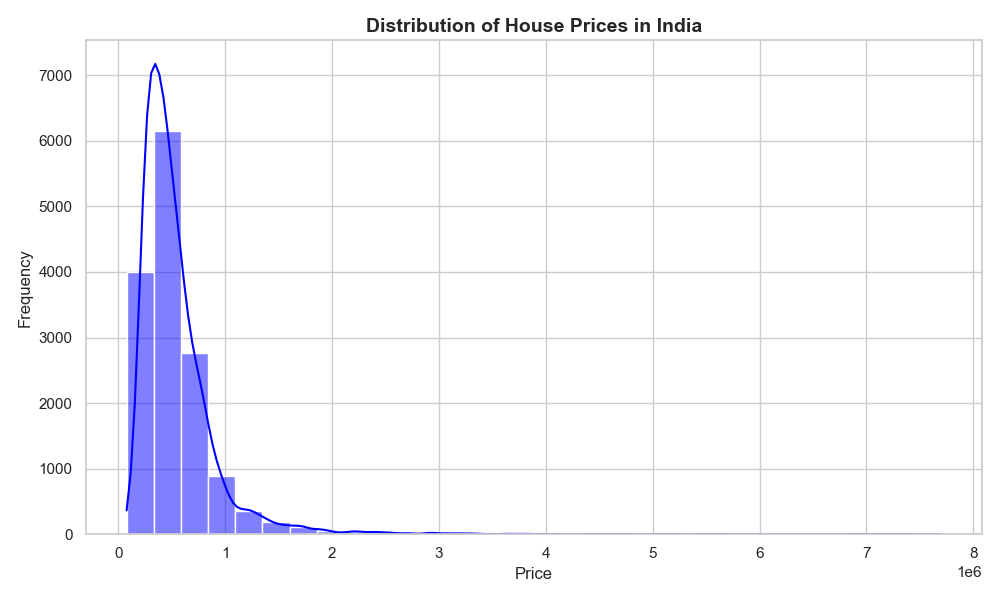
\includegraphics[width=\linewidth]{results/figures/price_distribution.png}
    \caption{Distribution of House Prices}
    \label{fig:price_distribution}
\end{figure}

\subsubsection{Univariate and Bivariate Analyses}
Key features such as \texttt{Number of Bedrooms}, \texttt{Living Area}, and \texttt{Bathrooms} were analyzed for their distributions and relationships with \texttt{Price}. Larger living areas and higher feature counts generally correlate with higher prices.

\begin{figure}[htbp]
    \centering
    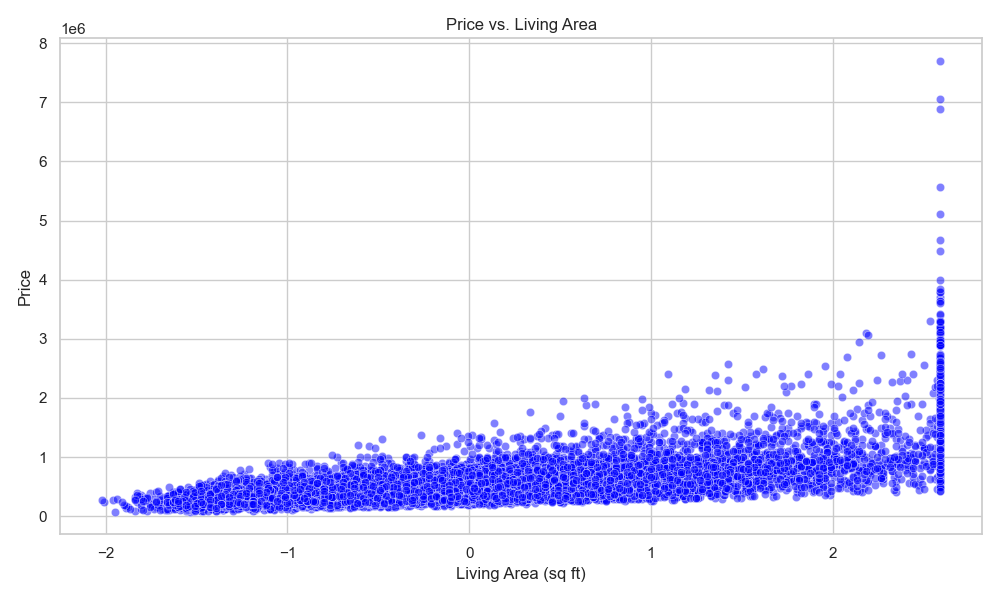
\includegraphics[width=\linewidth]{results/figures/price_vs_living_area.png}
    \caption{Price vs. Living Area}
    \label{fig:price_vs_living_area}
\end{figure}

\subsubsection{Data Cleaning and Feature Engineering}
Data cleaning involved imputing missing values, removing irrelevant columns, and handling outliers. New features such as \texttt{House\_Age}, \texttt{Time\_Since\_Renovation}, and \texttt{Total\_Area} were engineered to enhance predictive power.

\begin{itemize}
    \item \texttt{House\_Age}: Reflects property age.
    \item \texttt{Total\_Area}: Sum of living and basement areas.
\end{itemize}

\subsection{Correlation and Statistical Testing}

Correlation analysis revealed strong positive relationships between \texttt{Price} and features like \texttt{Living Area} (0.77) and \texttt{Grade}. Multicollinearity issues were identified between \texttt{Living Area} and \texttt{Total Area} (0.87), suggesting dimensionality reduction may be necessary.

\begin{figure}[htbp]
    \centering
    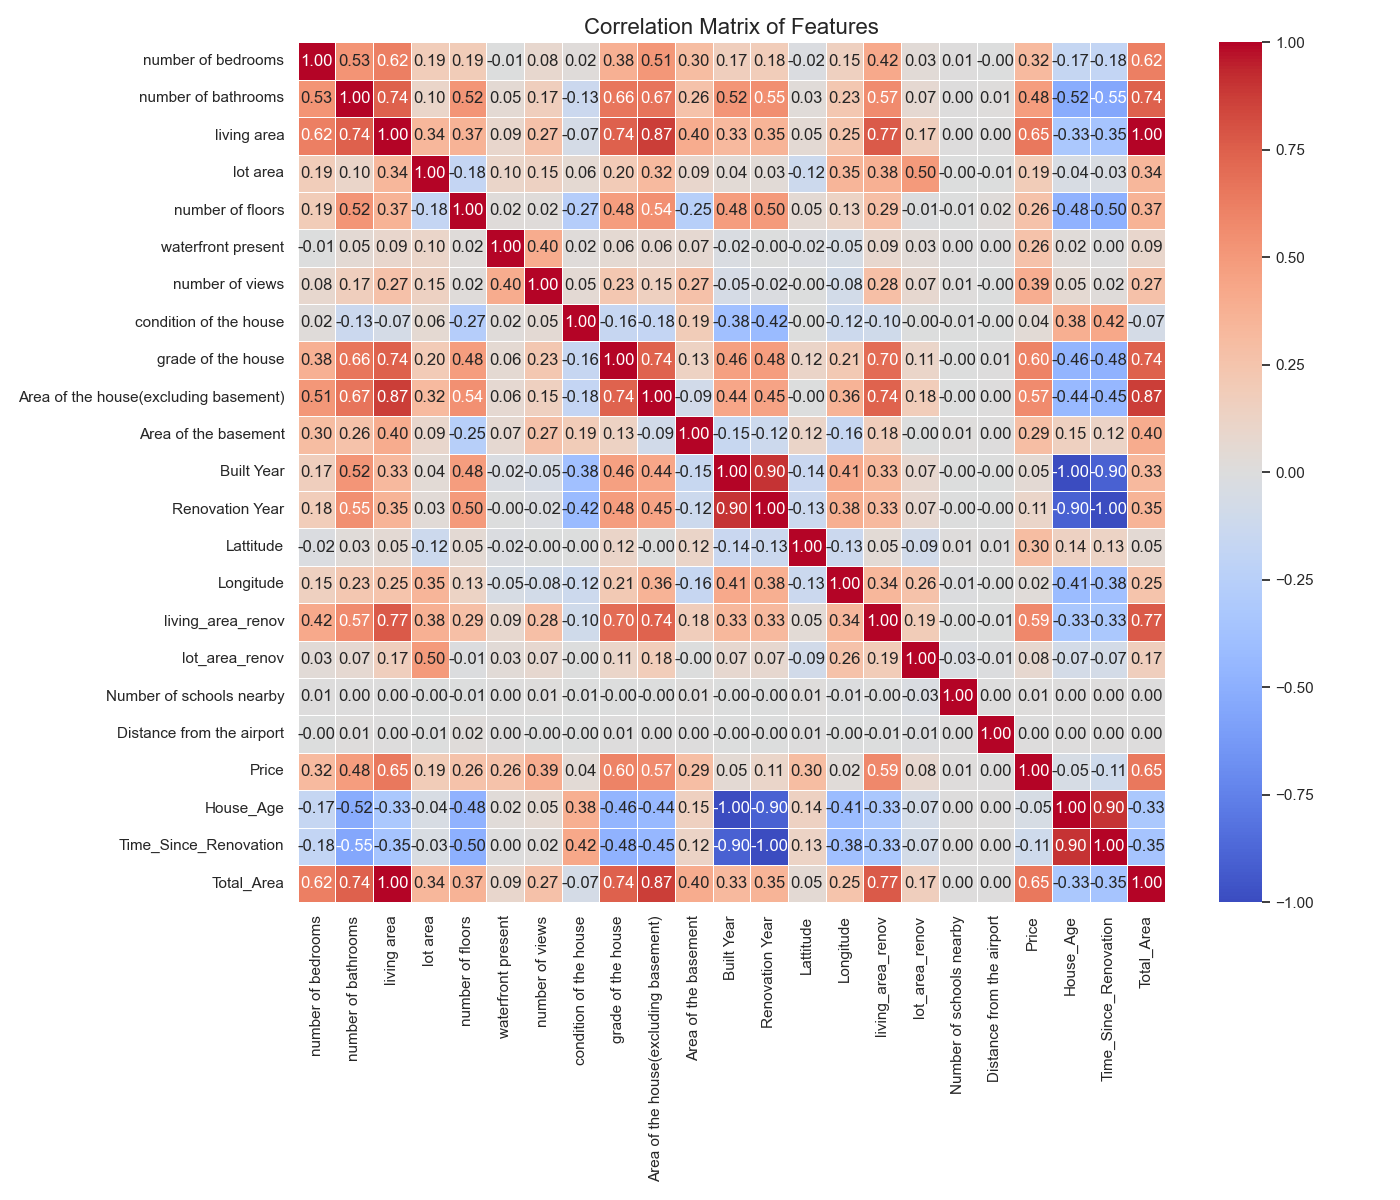
\includegraphics[width=\linewidth]{results/figures/correlation_matrix.png}
    \caption{Correlation Matrix Heatmap}
    \label{fig:correlation_matrix}
\end{figure}

Statistical tests confirmed significance for key features such as \texttt{Bathrooms} and \texttt{Waterfront Presence}. Insignificant features like \texttt{Distance from Airport} were excluded.

\subsection{Regression Modeling}

Ordinary Least Squares (OLS) regression explained 64.2\% of variability in \texttt{Price} (\(R^2 = 0.642\)). Significant predictors included \texttt{Total\_Area} and \texttt{Grade}. Multicollinearity issues were evident in certain features.

\begin{verbatim}
R-squared: 0.642
Significant Features: Total_Area, Grade, Bathrooms
\end{verbatim}

Model diagnostics highlighted non-linearity and heteroscedasticity in residuals, along with influential points identified via Cook's Distance.

\begin{figure}[htbp]
    \centering
    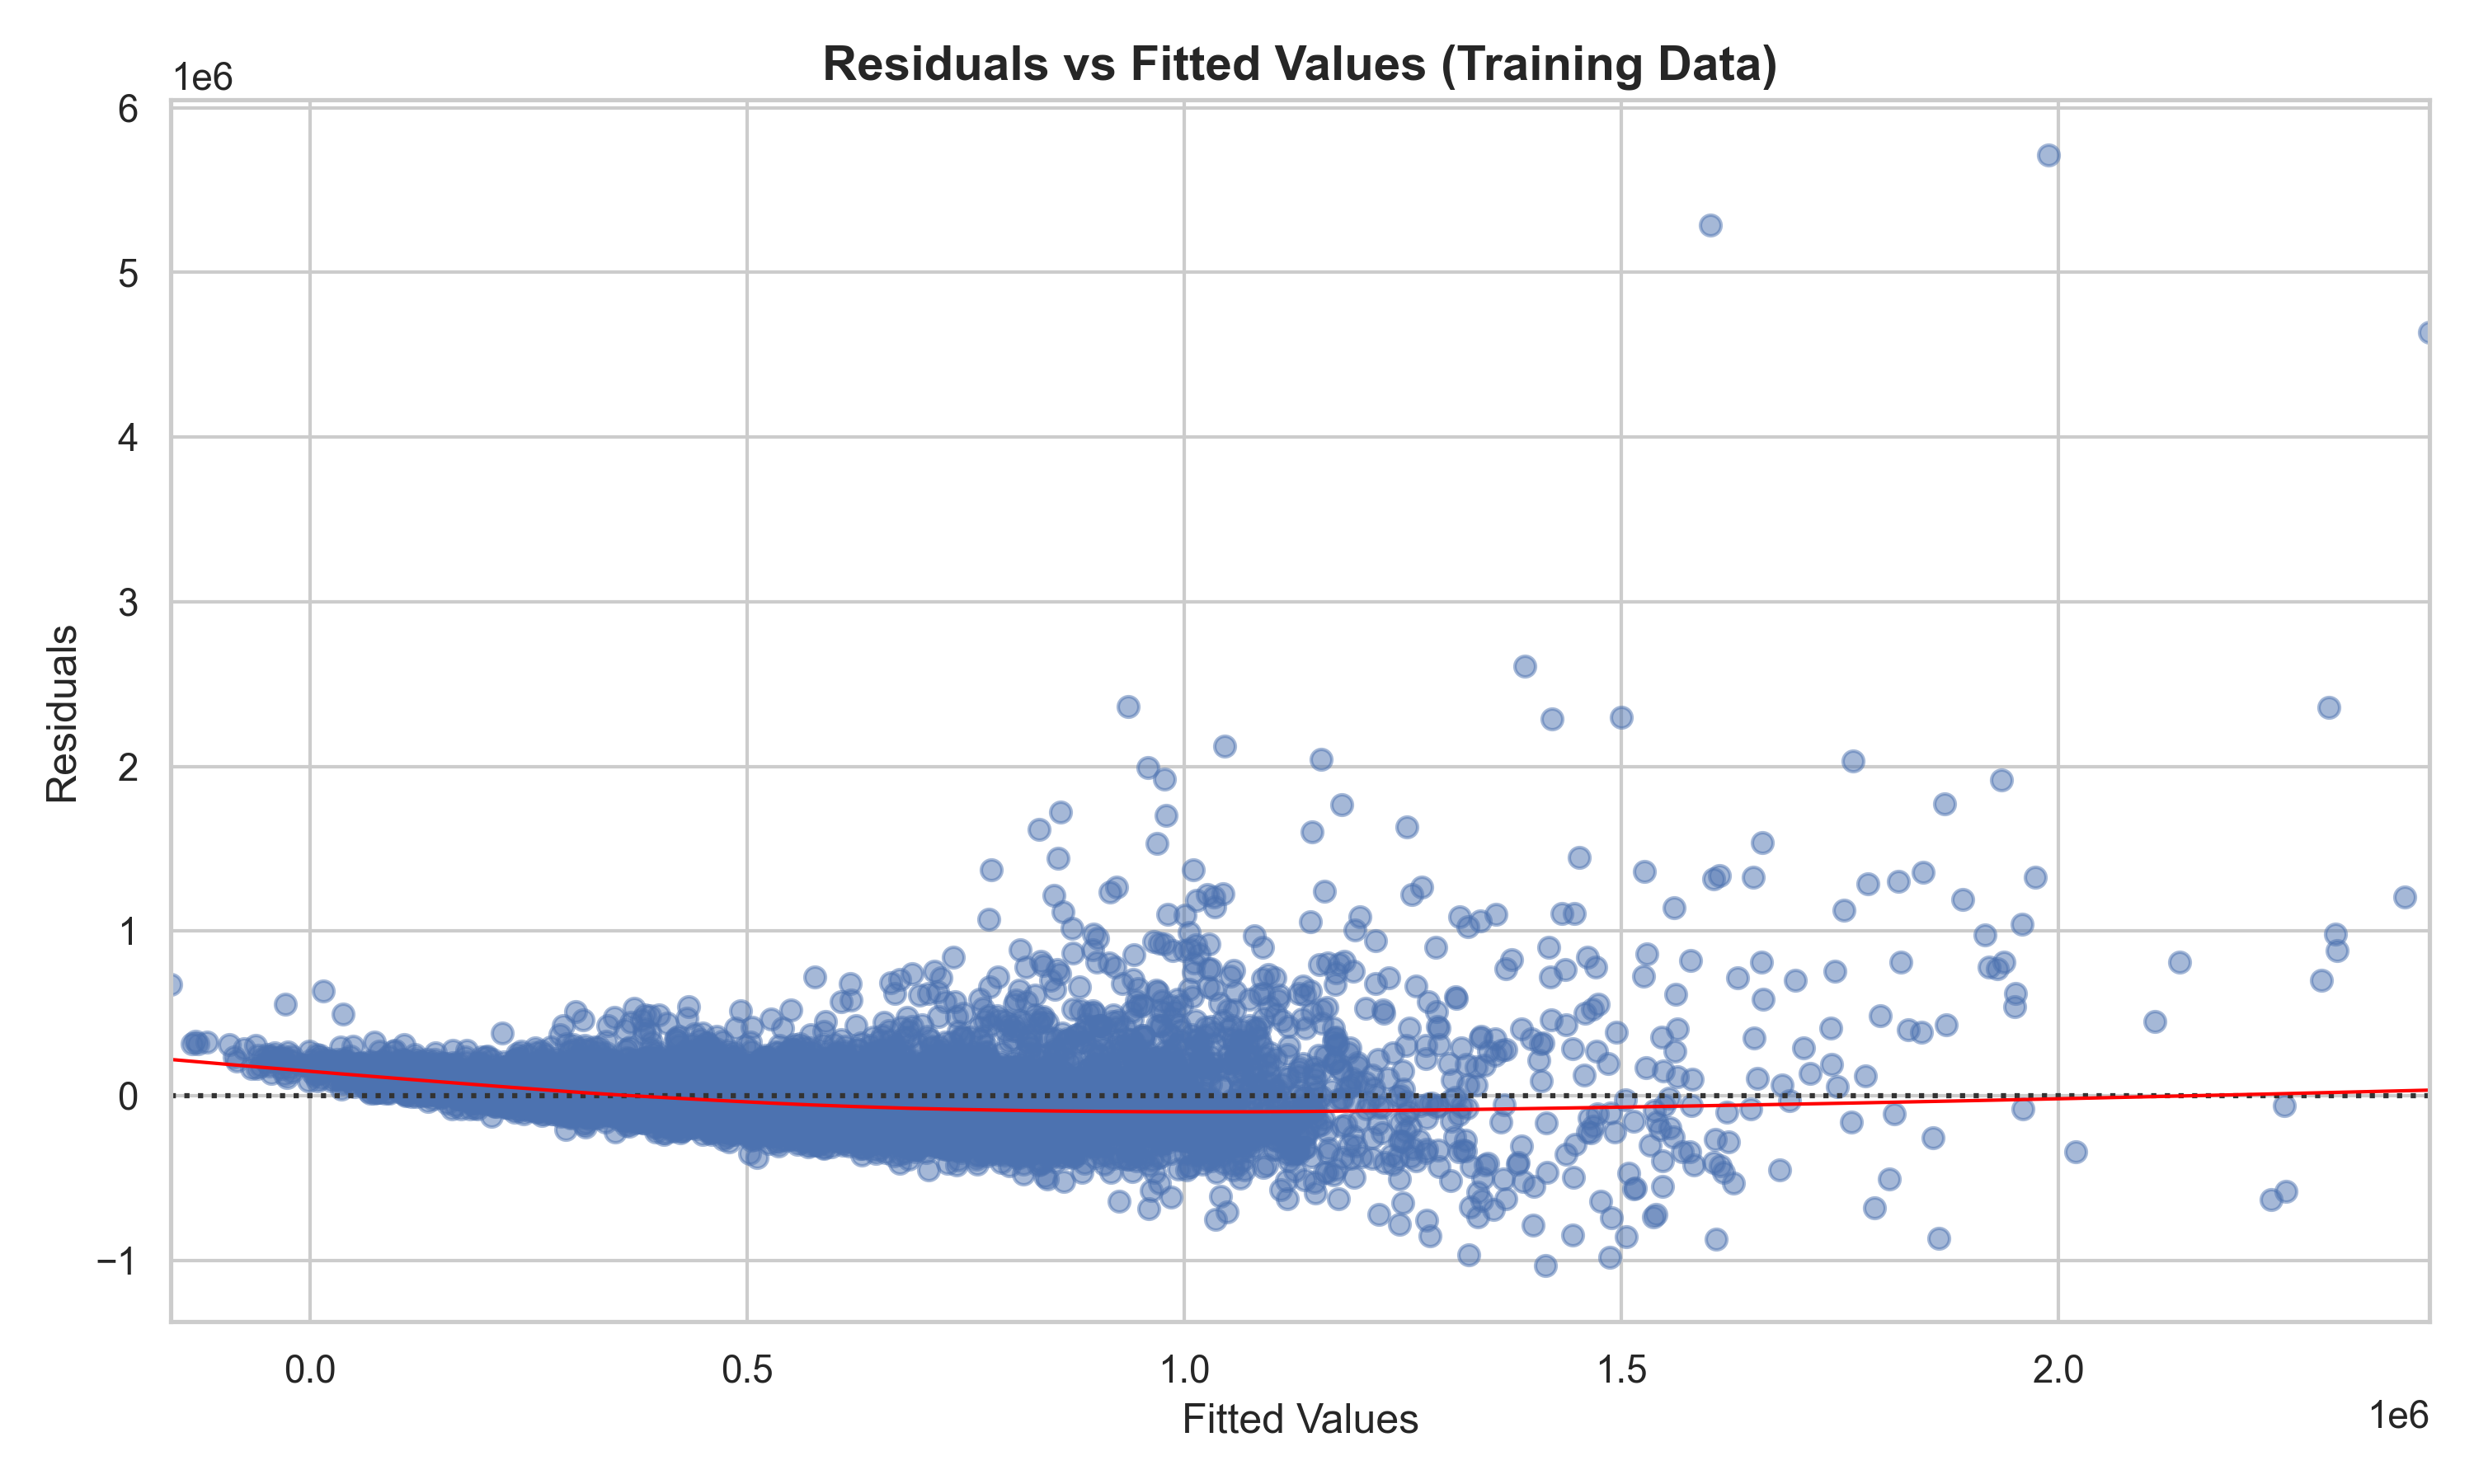
\includegraphics[width=\linewidth]{results/figures/residuals_vs_fitted_train.png}
    \caption{Residuals vs Fitted Values}
    \label{fig:residuals_vs_fitted_train}
\end{figure}

\subsubsection{Model Evaluation Metrics}
\begin{itemize}
    \item \textbf{MAE:} \$130,064
    \item \textbf{RMSE:} \$234,642
    \item \textbf{\(R^2\):} 0.63 (test data)
\end{itemize}
Despite reasonable accuracy, further refinement is needed to address multicollinearity and outliers.











\section{Methods}
\label{Methods}

\subsection{Pearson's Correlation}
\label{Pearsons-Correlation}

Pearson's correlation coefficient (denoted as \( r \)) measures the linear relationship between two continuous variables, ranging from \(-1\) to \(1\). A value of \( r = 1 \) indicates a perfect positive linear relationship, \( r = -1 \) indicates a perfect negative linear relationship, and \( r = 0 \) suggests no linear association. To test the significance of Pearson's correlation, a hypothesis test is conducted, where the null hypothesis (\( H_0 \)) states that there is no linear correlation in the population (\( \rho = 0 \)), and the alternative hypothesis (\( H_1 \)) posits a non-zero correlation. The test statistic is calculated as:
\[
t = r\sqrt{\frac{n-2}{1-r^2}},
\]
where \( n \) is the sample size. This statistic follows a \( t \)-distribution with \( n-2 \) degrees of freedom under the null hypothesis. By comparing the \( p \)-value obtained from this test to a predefined significance level (\( \alpha \)), we can determine whether to reject \( H_0 \) and conclude a statistically significant linear relationship between the variables.

\subsection{Multiple Testing Correction}
\label{Multiple-Testing-Correction}

In statistical analysis, conducting multiple hypothesis tests increases the risk of Type I errors, where a null hypothesis is incorrectly rejected. This issue arises because the probability of at least one false positive increases with the number of tests performed. To address this, multiple testing correction methods are employed to control the family-wise error rate (FWER), which is the probability of making one or more Type I errors across all tests.

One commonly used method for multiple testing correction is the \textit{Bonferroni method}. This approach adjusts the significance level \( \alpha \) by dividing it by the number of tests \( m \), resulting in an adjusted threshold:
\[
\alpha_{\text{adjusted}} = \frac{\alpha}{m}.
\]
A hypothesis test is deemed significant only if its \( p \)-value is less than \( \alpha_{\text{adjusted}} \). 

\subsection{Ordinary Least Squares and Testing Coefficients}
\label{OLS-and-Testing-Coefficients}

Ordinary Least Squares (OLS) is a fundamental method for estimating the parameters of a linear regression model. The OLS method minimizes the sum of the squared residuals, where residuals are the differences between the observed and predicted values of the dependent variable. For a linear regression model of the form 
\[
y = \beta_0 + \beta_1 x_1 + \beta_2 x_2 + \cdots + \beta_p x_p + \epsilon,
\]
OLS estimates the coefficients \( \beta_0, \beta_1, \ldots, \beta_p \) that best fit the data under the assumption that the error term \( \epsilon \) is normally distributed with mean zero and constant variance.

To test whether all regression coefficients except the intercept are zero, the \textit{F-test} is used. The null hypothesis for this test is 
\[
H_0: \beta_1 = \beta_2 = \cdots = \beta_p = 0,
\]
indicating that the independent variables do not collectively explain variation in the dependent variable. The alternative hypothesis is 
\[
H_1: \text{At least one } \beta_i \neq 0 \text{ for } i \geq 1.
\]

The test statistic is calculated as 
\[
F = \frac{\text{Explained Variance per Degree of Freedom}}{\text{Residual Variance per Degree of Freedom}},
\]
where the numerator represents the mean square regression (MSR), and the denominator represents the mean square error (MSE). This statistic follows an \( F \)-distribution with \( p \) and \( n-p-1 \) degrees of freedom under the null hypothesis, where \( n \) is the sample size. A low \( p \)-value from the \( F \)-test indicates that the regression model provides a significantly better fit to the data than a model with no predictors, allowing us to reject \( H_0 \) and conclude that at least one coefficient is non-zero.

\section{Discussion}

The findings of this study provide valuable insights into the factors influencing house prices and the challenges inherent in predictive modeling for real estate. 

\subsection{Interpretation of Results}

Our analysis confirmed that structural features like \texttt{Total\_Area}, \texttt{living area}, and \texttt{grade of the house} are the most significant predictors of house prices, reflecting their central role in determining property value. Additional features, such as \texttt{waterfront presence} and \texttt{Renovation Year}, highlight the importance of location and property condition. Conversely, features like \texttt{House\_Age} and \texttt{Time\_Since\_Renovation} negatively impacted prices, consistent with market tendencies that favor newer or recently renovated properties.

Despite reasonable predictive performance, the Ordinary Least Squares (OLS) regression model encountered challenges in accurately modeling higher-priced properties. This is evident in the heteroscedasticity observed in residual analysis and the model's underestimation of extreme price variations. These results underscore the complexity of real estate markets, where unique and high-value properties often deviate from general trends.

\subsection{Model Limitations}

Several limitations were identified, including multicollinearity among highly correlated features (\texttt{Total\_Area}, \texttt{living area}), which may have destabilized coefficient estimates. Heteroscedasticity and non-normal residuals suggest that the model assumptions of linearity and constant variance were not fully met. Additionally, the influence of 499 outlier observations, as identified through Cook's Distance, highlights the impact of data variability on model robustness.

The exclusion of features such as \texttt{Longitude} and \texttt{Distance from the airport}, due to their low predictive value, points to potential shortcomings in the dataset's granularity or feature representation. Incorporating neighborhood-level factors or temporal market trends may improve feature relevance and model accuracy.

\subsection{Broader Implications}

The study demonstrates the importance of data quality, feature engineering, and rigorous diagnostic testing in building predictive models for house prices. It also highlights the trade-offs between model simplicity and the ability to capture complex, non-linear relationships inherent in real estate data. These findings can inform future research and practical applications in real estate analytics, particularly in designing models that balance interpretability and predictive performance.

\subsection{Future Directions}

Building on these findings, future research should explore advanced modeling techniques, such as tree-based algorithms (e.g., Random Forest, Gradient Boosting) or regularization methods (e.g., Ridge, Lasso), to handle multicollinearity and improve robustness. Addressing heteroscedasticity through transformations or heteroscedasticity-consistent standard errors may further enhance model validity. Finally, incorporating external data sources, such as demographic trends and economic indicators, can provide a more holistic view of the factors influencing house prices.

This study lays the groundwork for more refined and adaptive approaches to real estate price prediction, with implications for both academic research and practical decision-making.

\section{Conclusion}

\subsection{Key Determinants of House Prices}

The analysis highlights \texttt{Total\_Area}, \texttt{living area}, and \texttt{grade of the house} as the strongest positive contributors to house prices, reflecting the premium on larger and higher-quality properties. Features like \texttt{waterfront present} and \texttt{Renovation Year} also positively influence prices. Conversely, older homes and properties with longer times since renovation (\texttt{House\_Age} and \texttt{Time\_Since\_Renovation}) show negative impacts, emphasizing the importance of property condition.

\subsection{Model Performance}

The Ordinary Least Squares (OLS) regression model explained 64.2\% of price variability (\(R^2 = 0.642\)), with a test set MAE of \$130,064 and RMSE of \$234,642. While the model performed reasonably well, residual analysis revealed underperformance for higher-priced properties, highlighting areas for improvement.

\subsection{Limitations}

Key limitations include multicollinearity among features (\texttt{Total\_Area} and \texttt{living area}), heteroscedasticity in residuals, and deviations from normality. Influential points identified by Cook's Distance (499 observations) disproportionately affected the model, and certain features (\texttt{Longitude}, \texttt{Distance from airport}) were insignificant, likely due to data quality or granularity.

\subsection{Future Work}

To improve the model, future efforts should:
\begin{itemize}
    \item Address multicollinearity through feature selection or dimensionality reduction (e.g., PCA).
    \item Apply transformations (e.g., log) to normalize residuals and stabilize variance.
    \item Explore advanced models such as Lasso regression or tree-based algorithms to capture non-linear relationships.
    \item Enhance feature representation by incorporating neighborhood-level factors and market conditions.
\end{itemize}

By addressing these areas, future models can provide more accurate predictions and deeper insights into the determinants of house prices.



\nocite{*}
\printbibliography
\end{document}